%TEX root = ../dissertation.tex

\chapter{Background}
\label{chapter:background}

In this chapter, it is first introduced some general concepts about Binary
Decision Diagrams which will be used later on inference methods of logical
programming languages, followed by an introduction to Markov Decision Processes
and their generalization for partially observable environments, describing
domains like the one being studied. Afterwards, it is initiated the study on
logical programming languages and their specialization to a probabilistic model,
which will be the basis for making decisions in planning problems.

\section{Binary Decision Diagram}
In this chapter, it is showed a relevant data structure for representing Boolean
functions that is used in some of the inference mechanisms for probabilistic
logic programming languages.

A \textit{Binary Decision Diagram (BDD)} \cite{Andersen1999} is a rooted,
directed acyclic graph with one or two terminal nodes and without any children
labeled 0 or 1. In this graph, all the remaining variable nodes, individually
labeled as $\lambda$, have out-degree two. Each $var(\lambda)$ represents a
variable node and has two outgoing edges given by functions $low(\lambda)$ and
$high(\lambda)$.

In a diagram, dotted lines represent Low-edges, leaving High-edges with
solid lines. In the figure \ref{fig:bdd_grp}, we can see an example of a
\textit{BDD} for a specific boolean function.

\begin{figure}[H]
    \centering
        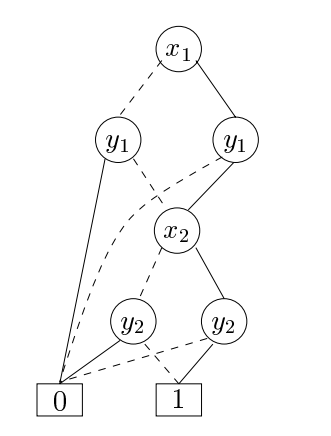
\includegraphics[width=5cm]{images/first_bdd}
        \caption{Example of a \textit{BDD} with the boolean function: $ (x_1
        \Leftrightarrow x_2) \wedge (x_2 \Leftrightarrow y_2) $
        \cite{Andersen1999} }
        \label{fig:bdd_grp}
\end{figure}

As we will see further down the road, this \textit{BDD} can be used to model
the best action an agent can take to maximize its expected utility.

\section{Markov Decision Process}

Assuming an agent is interacting with an environment and has to
make sequential decisions on a world that is fully observable with outcomes
of its actions that have a stochastic behaviour and the transition from one
state to another only depend on the current state (\textit{Markovian}
Transitions) with additive rewards, we can classify this problem as a \textit{
Markov Decision Process (MDP)} \cite{Russell2009} defined by the following:
\begin{itemize}
    \item Set $\textbf{S}$, the state space; the total possible states an agent
    can be in.
    \item Set $\textbf{A}$, the action space; all possible actions the agent can
    perform.
    \item Transition Function $\textbf{T}:S \times A \times S \to [0,1]$, which
    is equivalent to $p(s'|s,a)$, the probability of reaching state $s'$ from
    state $s$ by performing action $a$.
    \item Reward Function $\textbf{R}: S \times A \to \mathbb{R}$, which
    translates to the reward the agent is given by performing action $a$ in
    state $s$\footnote{The reward function can also depend on the outcome of
    executing action $a$, but here we stuck with the simplified version of it.}.
    \item Discount factor $ \gamma \in [0,1]$, representing the difference
    between present and future rewards.
\end{itemize}

So a \textit{MDP} can be summarized as a tuple $(\textbf{S, A, T, R},\gamma)$,
where the solution to this problem is the set of decisions the agent will make
for any state he can reach. This is normally referred as a \textit{policy}
(represented by $\pi(s)$). Thus, even if the outcome of an action is not what
would be expected, the agent will always know what action he must perform in
that state. The agents' policy will be the one that yields the highest expected
utility, the \textit{optimal policy} ($\pi^*(s)$). In this way, the goal is
to infer policy $\pi : \textbf{S} \times \textbf{D} \to \textbf{A}$ over the
time period (\textit{d steps}) in which our agent is expected to run, for each
state \textit{s}, hence we can sample the time period in a finite number of time
steps $ t = 0, 1, ..., T$ (\textit{finite horizon}) to get the
\textit{value function} (\textit{V}-function):
\begin{equation}
    \label{eq:reward}
    V_d^\pi(s_t) = \mathbb{E}[\displaystyle\sum_{k=t}^{t+d} \gamma^{k-t}R(s_k,
    a_k)|s_t,\pi]
\end{equation}

The optimal policy is the set of actions in each state that maximize equation
\ref{eq:reward}. The equation above can be extended to compute the expected
reward under the optimal policy. This equation is called the
\textit{action-value function} (\textit{Q}-function):
\begin{equation}
    \label{eq:qreward}
    Q_d^\pi(s_t,a_t) = \mathbb{E}[\displaystyle\sum_{k=t}^{t+d}
    \gamma^{k-t}R(s_k,a_k)|s_t,a_t,\pi]
\end{equation}

In figure \ref{fig:dbn_mdp} there is an example of a \textit{MDP} modeled as
a \textit{Dynamic Bayesian Network} (\textit{DBN}), useful to explain how a
process of this genre behaves.

\begin{figure}[H]
    \centering
        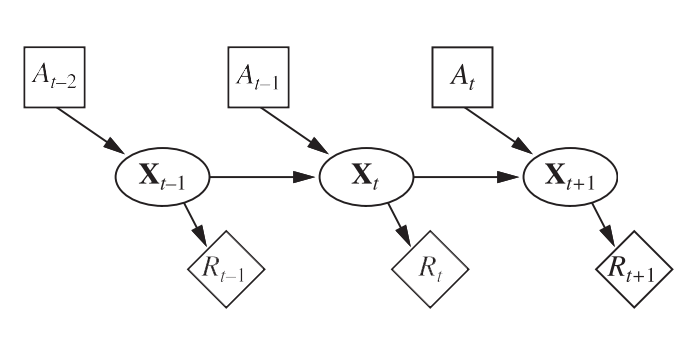
\includegraphics[width=8cm]{images/mdp-dbn}
        \caption{Example of a \textit{DBN} representation of a
        \textit{MDP}. Adapted from \cite{Russell2009}.
        }
        \label{fig:dbn_mdp}
\end{figure}

In a \textit{MDP}, it is common to have an exponential number of states, making
it impossible to calculate the expected reward of a policy. Thus, one way to
solve them in a reasonable manner is to establish a fixed number of runs and
in each one of them, estimate the value function for the policy found (this is
called a partial policy).
By using this procedure, the initial state of each run will be the final state
that resulted from the execution of the previous one and it finishes when a
terminal state is reached.

Classical procedures exist for solving these kind problems using iterative
procedures. One of them calculates the utility of each state, using its
neighbors', and the other takes turns to calculate the states' utilities with
the present utility and to improve its own state policy with all the current
utilities. The first one is called \textit{Value Iteration} and the latter is
referred to as \textit{Policy Iteration}.
They are broadly discussed in \cite{Russell2009}.

\subsection{Partially Observable Markov Decision Process}
When the state is fully determined by the agent, we can calculate the policy
for each state an agent can be. However, this assumption is not valid when the
agent is not sure on his current state. So the previous model can be extended
to partially observable environments, \textit{Partially Observable Markov
Decision Processes} \cite{Russell2009} (\textit{POMDP}). They occur much more
frequently than the previous type of problems and are usually harder to solve.

To characterize a process of this genre, it must be defined as having the same
tuple that \textit{MDP's} had with the addition of:
\begin{itemize}
    \item Set $\Omega$, the observation space, the total possible
    observations given by the world.
    \item Observation function $\textbf{O}: \Omega \times S \times
    A \to [0,1]$, represented by $ O(a,s',o) = P(o|s',a)$, meaning the
    probability of obtaining observation $o$ by reaching the new state $s'$ and
    have performed the action $a$.
\end{itemize}

As the current state is not directly available to the agent, it must behave
accordingly with its belief state ($b$), the set of actual states the agent
might be in, which can grow exponentially with the number of states. This
translates to a probability distribution over all states.
This belief is given equation \ref{eq:pomdps1}, where $s'$ is the new state
reached from performing action $a$ when in state $s$, given the evidence $e$
($\alpha$ is just a normalizing constant to make belief states sum to 1).
\begin{equation}
    \label{eq:pomdps1}
    b'(s') = \alpha P(e|s')\displaystyle\sum_{s} P(s'|s,a)b(s)
\end{equation}

Now, a very important assumption can be made, the optimal action does not depend
on the actual state the agent is in, only on the agent's current belief state.
Thus, the optimal policy will be applied to the belief, $\pi^{*}(b)$, so that
the agent can map belief states to actions.

The \textit{Value}-function can be adapted from \ref{eq:reward} to introduce the
contribution of the belief.
\begin{equation}
    \label{eq:pomdpreward}
    V_d^\pi(b_t) = \mathbb{E}[\displaystyle\sum_{k=t}^{t+d} \gamma^{k-t}R(s_k,
    a_k)|b_t,\pi]
\end{equation}

By extending the diagram from \ref{fig:dbn_mdp}, it can be obtained the \textit{
DBN} representing the POMDP, in figure \ref{fig:dbn_pomdp}.

\begin{figure}[H]
    \centering
        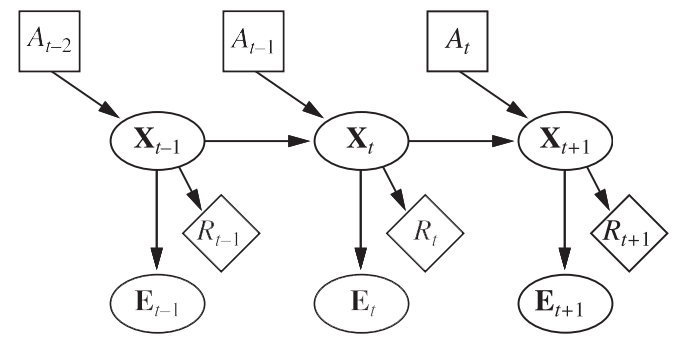
\includegraphics[width=8cm]{images/pomdp-dbn}
        \caption{Example of a \textit{DBN} representation of a
        \textit{POMDP}. Adapted from \cite{Russell2009}.
        }
        \label{fig:dbn_pomdp}
\end{figure}

Summarizing, as a \textit{POMDP} can have a very large number of states (which
generally happens) and the current state is only partially observable, the agent
must resort to beliefs. Hence, the existence of an ordered plan made by an agent
in this kind of processes is not viable. So the agent must use policies over
beliefs.

\section{Prolog}

Prolog is a logical programming language introduced by Alain Colmerauer and
Philippe Roussel \cite{Colmerauer1993,prolog} that was designed to simulate
the man-machine communication system in natural language. The goal was also to
integrate logic as a declarative knowledge representation language with a
procedural representation of knowledge.

As it is said before, what makes this programmming language different than the
others is the fact that it is declarative, it does not describe the control flow
of the program, only the logic of the computation. This logic is expressed by
means of relations between objects, and its execution is started by running a
query over the knowledge base of relations. Relations are rules, represented by
an implication clause with an \textit{Head} and a \textit{Body}, using the
appropriate predicates.
\begin{gather*}
    Head :- Body. \\
    Body \Rightarrow Head
\end{gather*}
Facts can also be modeled as rules, that is grounded clauses with an empty
\textit{Body}.
% ------- %
\begin{center}
\begin{tabular}{c}
    \lstinputlisting[
      language = Prolog,
    ]{chapters/script/p1.pl}
\end{tabular}
\end{center}
The ensemble of facts, rules and queries are built out of terms, its single data
type. Terms can be complex or simple, if they are composed by variables or
constants (Atoms or Numbers).

New rules can be created by joining a combination of facts, increasing the
information about the world. A query provided to the prolog interpreter is
handled through this rules using the Unification-Resolution mechanism with a
backtracking flow model control, returning 'Yes', if the solver can prove the
query clause with all the remaining clauses in the database, or 'No', if the
solver cannot prove it with the available information about the world.

Prolog is built upon the \textit{Closed World Assumption}, which says that all
knowledge about the world is present in the database. If some term is not in the
database, its value is assumed to be false. The result provided by the
interpreter must be seen as an attempt of the programming language to prove that
the asked query is true in some model of the world. So if the solver returns a
'No' answer, it does not necessarily mean that the query clause is false, just
that the solver cannot prove it with the available information about the world.

A simple prolog example relevant to the problem that is being treated can be
seen in Appendix \ref{code:prolog}.

\subsection{ProbLog}
In this section, it is introduced Probabilistic Prolog (ProbLog\footnote{Full
documentation, examples and support are available at
\url{https://dtai.cs.kuleuven.be/problog/}}) \cite{Kimmig2011,DeRaedt2007}, an
expansion over the classic Prolog language, where a program specifies a
distribution of its non-probabilistic subprograms. All facts are
labeled with probabilities and behave like mutually independent random
variables, specifying if some fact belongs to a random sampled program.
If there is more than one grounded instance of the same predicate, then
they are also independent random variables.

A typical query in \textit{ProbLog} will not be prooved, it will be inferred its
success probability.

So, to write a ProbLog program, it is necessary to describe the set of labeled
facts $p_i :: c_i$, where each fact $c_i$ has a probability $p_i$ of being true,
and the remaining definite clauses, which adds the Background Knowledge
(\textit{BK}).

By having a ProbLog program $T = \left\{ p_1 :: c_1, ..., p_n :: c_n \right\}$
and some \textit{BK} with a finite set of possible substitutions
$\left\{ \theta_{j1}, ..., \theta_{ji_j}  \right\}$ for each probabilistic fact
$p_j :: c_j$, the maximum set of logical facts which can be added to \textit{BK}
are $L_T = \left\{ c_1\theta_{11}, ..., c_1\theta_{1i_1}, ..., c_n\theta_{n1},
..., c_n\theta_{ni_n} \right\}$. In fact, this program defines a probability
distribution over ground logic programs $L \subseteq L_T$ with:
\begin{equation}
    P(L|T) = \displaystyle\prod_{c_i\theta_j \in L} p_i
    \displaystyle\prod_{c_i\theta_j \in L_T \setminus L} (1-p_i)
\end{equation}

Now that is perfectly clear how ProbLog treats facts and rules, it makes sense
to talk about the mathematical meaning of a general query. So, the
probability of success of a query $q$ is given by:
\begin{equation}
    \label{eq:query_success}
    P_s(q|T) = \displaystyle\sum_{L \subseteq L_T} P(q|L)P(L|T),
\end{equation}
Where $P_s(q|T)$ is the marginal of $P(L|T)$ with respect to a query $q$ and:
\begin{itemize}
    \item $P(q|L) = 1$ if $L \cup BK \models q\theta$ for some value of
    $\theta$.
    \item $P(q|L) = 0$ otherwise.
\end{itemize}

It can also be asked the \textit{explanation} of some query $q$, that is the
probability of a specific proof \textit{E}. This \textit{explanation} is the
minimal subset of probabilistic facts and its \textit{BK} that entails $q\theta$
for some substitution of $\theta$, where $E(q)$ are all the minimal sets $E
\subseteq L_T$ of probabilistic facts such that $E \cup BK \models q$.
This means that:

\begin{equation}
    P(E|T) = \displaystyle\sum_{L \subseteq (L_T \setminus E)} P(L \cup E|T) =
    \displaystyle\prod_{c_i \in E} p_i
\end{equation}
Finally, the explanation probability is the most likely explanation or proof of
the query $q$.
\begin{equation}
    P_x(q|T) = max_{E \in E(q)} P(E|T) = max_{E \in E(q)}
    \displaystyle\prod_{c_i \in E} p_i
\end{equation}

As the equations above indicate, the calculations needed to answer a query
increase exponentially with the number of probabilistic facts, making the
inference mechanism the bottleneck of the programming language. It has been
investigated in \cite{Kimmig2011} exact and approximate inference algorithms and
their performances.

In appendix \ref{code:problog}, it can be seen an example\footnote{It is
important to refer that the version used for inference was \textit{ProbLog2}.}
of a program written in \textit{ProbLog}, continuing with the discussion started
with appendix \ref{code:prolog}.
